\documentclass[11pt]{beamer}

\usetheme{metropolis}

\usepackage{graphicx}
\usepackage{physics}
\usepackage{adjustbox}
\usepackage{caption}
\usepackage{chemformula}
\usepackage{quoting}
\usepackage[style=chem-angew,backend=bibtex]{biblatex}
\bibliography{references}
%
% Choose how your presentation looks.
%
% For more themes, color themes and font themes, see:
% http://deic.uab.es/~iblanes/beamer_gallery/index_by_theme.html
%
\mode<presentation>
{
  \usetheme{default}      % or try Darmstadt, Madrid, Warsaw, ...
  \usecolortheme{default} % or try albatross, beaver, crane, ...
  \usefonttheme{default}  % or try serif, structurebold, ...
  \setbeamertemplate{navigation symbols}{}
  \setbeamertemplate{caption}[numbered]
  \setbeamerfont{footnote}{size=\tiny}
} 

\usepackage[english]{babel}
\usepackage[utf8]{inputenc}
\graphicspath{{../lectureMW/image/}}

\AtBeginSection[]{
\begin{frame}{Outline}
  \tableofcontents[currentsection]
\end{frame}
}

\title{Chapter 5: Chemical Reactions and Equations}
\institute{Chemistry Department, Cypress College}
\date{September 26, 2022}

\begin{document}

\begin{frame}
  \titlepage
\end{frame}

\begin{frame}{Class Announcements}
  \textbf{Lecture Section}
  \begin{itemize}
  \item All assignments have been graded
  \item 1.5 hrs Ch. $1 - 4$ exam, questions are based on the lectures,
    homework, and worksheets
  \item Review Ch. 4 material and begin Ch.5 - Chem Reactions and Equations
  \end{itemize}
\end{frame}

\section{Review: Mass Percent, Moles, and Molarity}

\begin{frame}{Elemental Composition of a Penny}
  \begin{center}
    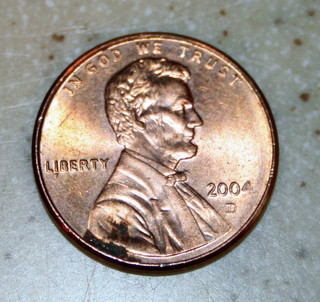
\includegraphics[scale=0.3]{penny_2004}
  \end{center}

  \begin{itemize}
  \item Penny has not been made of solid copper
  \item Mix of cheaper metal along with copper on the surface
  \item Made of $97.5\%$ zinc and $2.5\%$ copper
  \end{itemize}
\end{frame}

\begin{frame}{Different Types of Steel}
  \begin{center}
    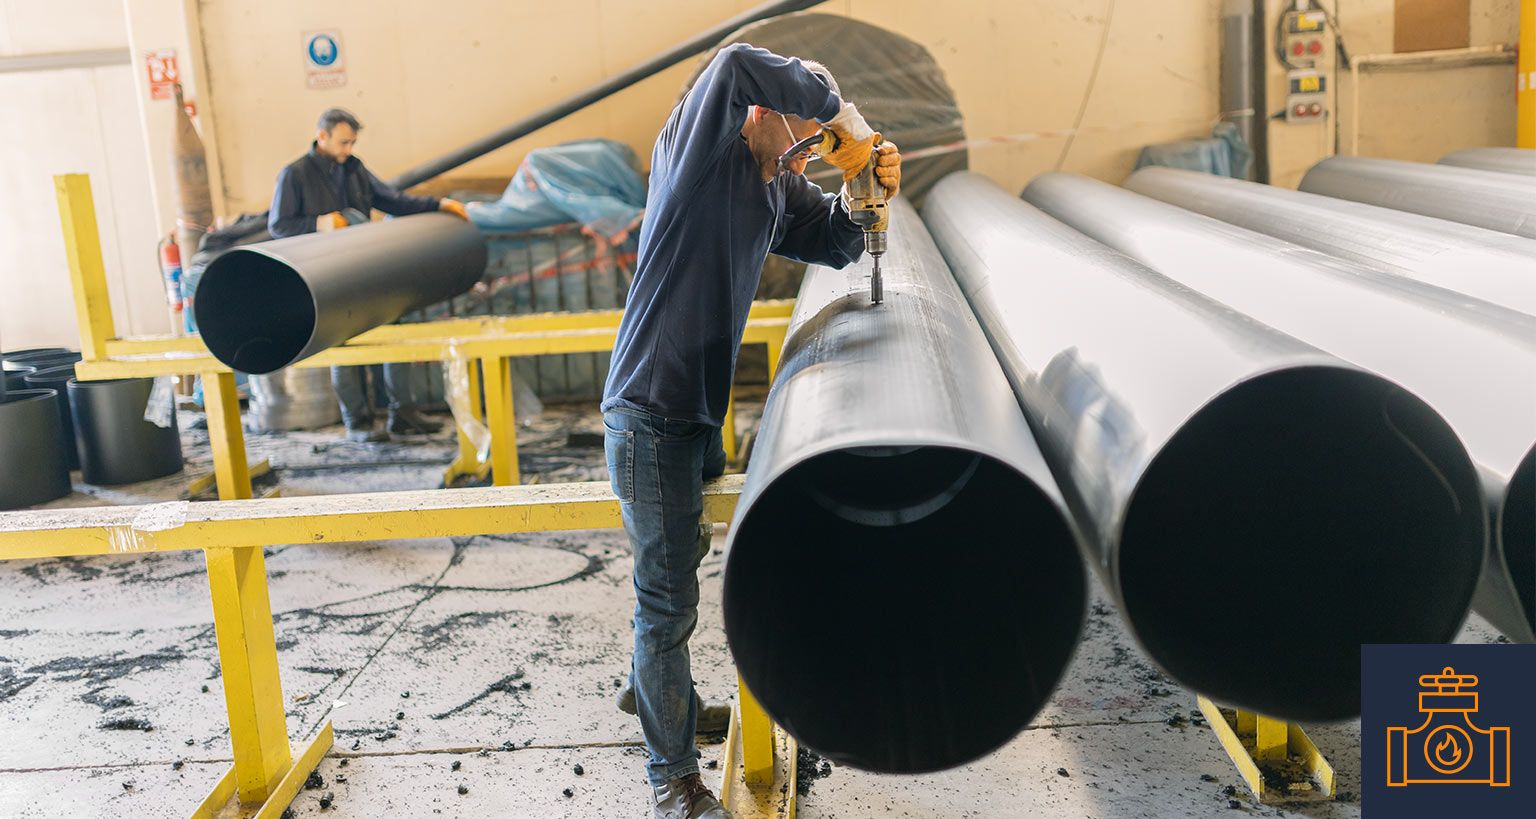
\includegraphics[scale=0.12]{steel_type}
  \end{center}

  \begin{itemize}
  \item Steel is a metal alloy; mixture of different
    metals yield different physical properties
  \item Different types:
    \begin{itemize}
    \item Carbon steel
    \item Stainless steel
    \item Alloy steel
    \item Tool steel
    \end{itemize}
  \end{itemize}
\end{frame}

\begin{frame}{Mass Percent Composition}
  \textbf{Main Takeaway:} Convert the mass of each component
  to a percentage of the total mass

  \begin{equation}
    P_A = \frac{M_A}{M_\text{Tot}} \times 100\%
  \end{equation}

  where $M_\text{Tot}$ is the total mass, $M_A$ is the mass and $P_A$
  is the percent composition for component $A$  
\end{frame}

\begin{frame}{The Mole Concept}
  \begin{center}
    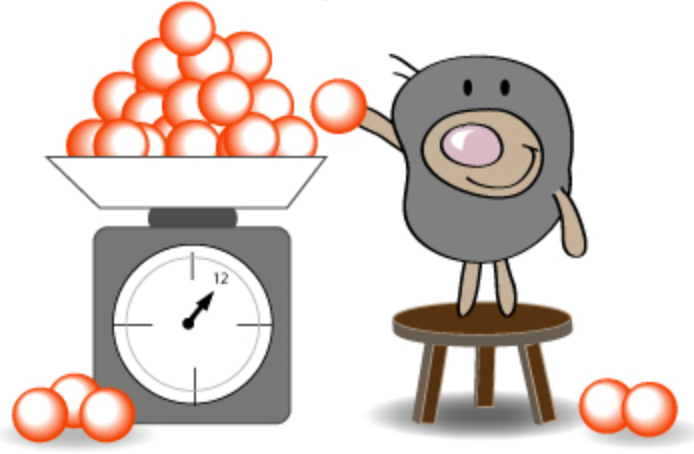
\includegraphics[scale=0.2]{mole}
  \end{center}
  
  \textbf{Q:} What is a mole (mol)?

  \textbf{A:} A mole is measurement of a substance and relates to
  Avogadro's number ($6.022 \times 10^{23}$ molecules/mol)

  \textbf{side note:} Mole day is Oct. 23, between 6:02 a.m. and 6:02 p.m
\end{frame}

\begin{frame}{Purpose of the Mole}
  \begin{center}
    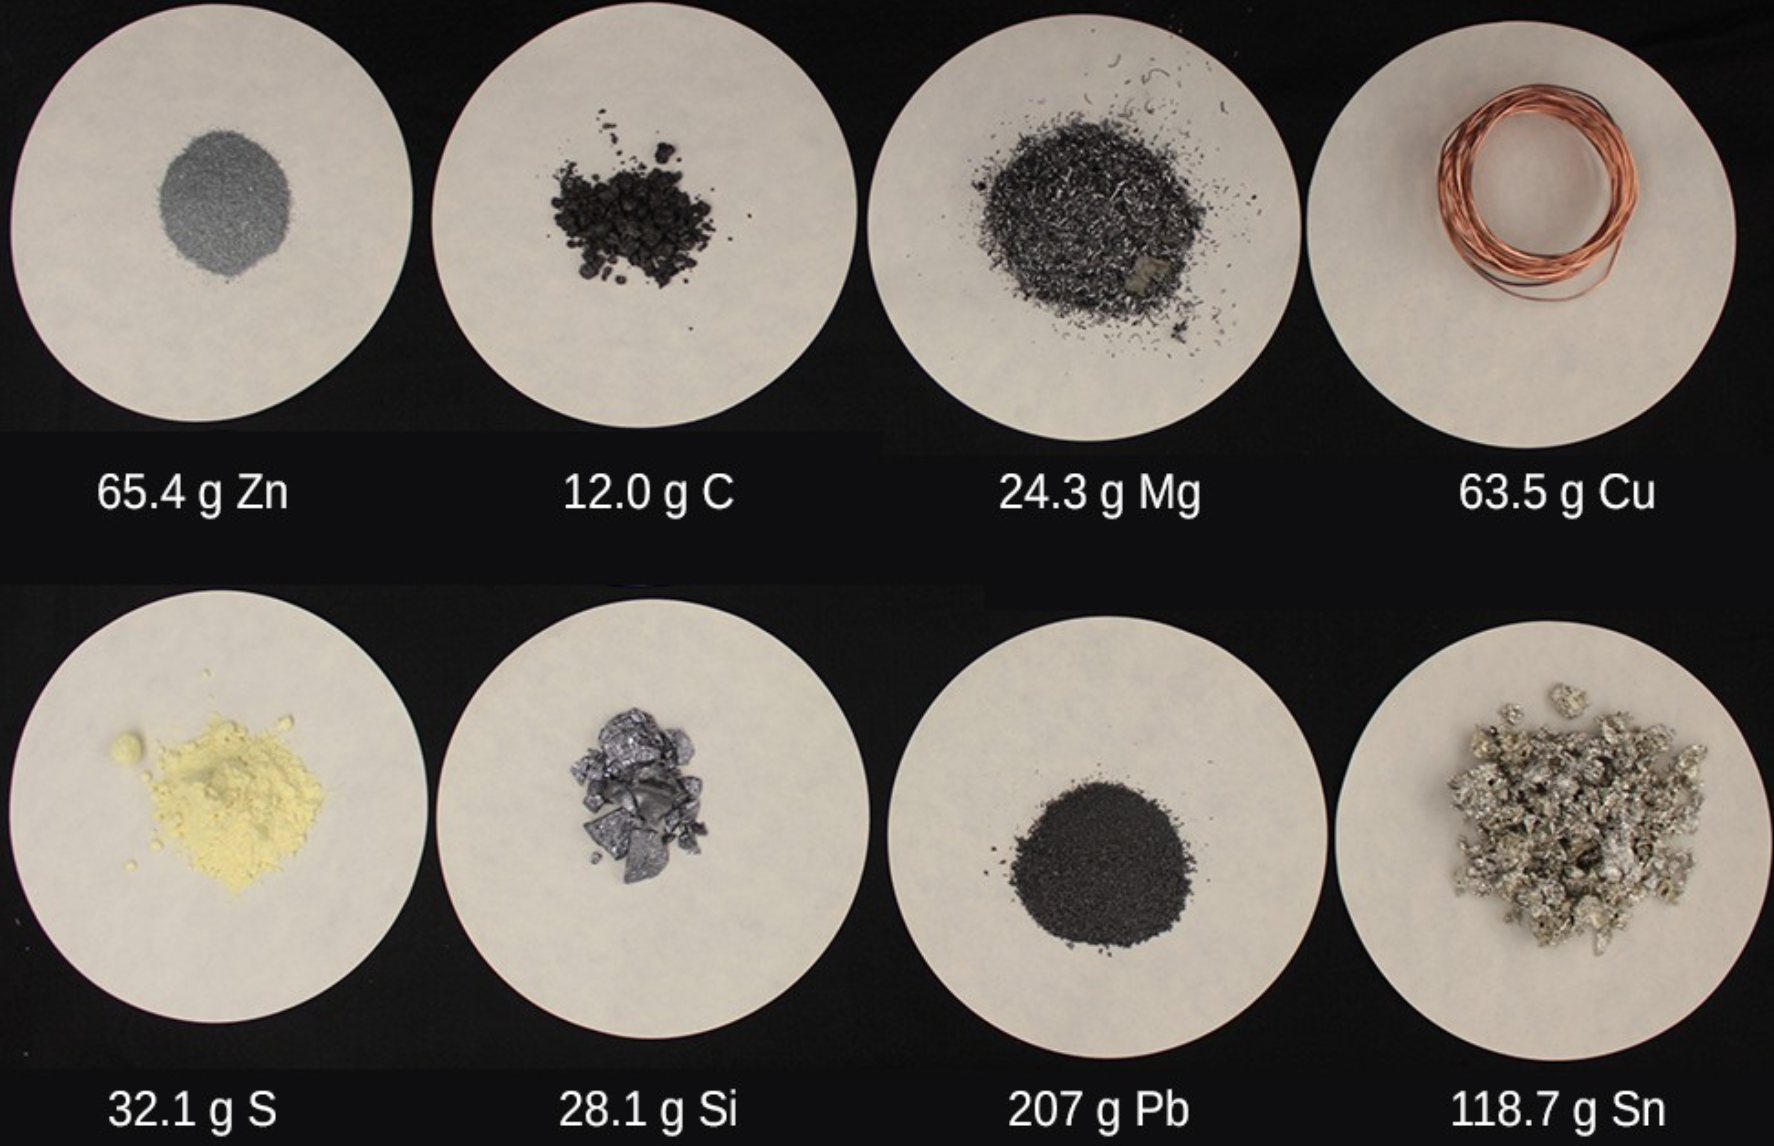
\includegraphics[scale=0.1]{mol_solids}
  \end{center}
  
  \begin{itemize}
  \item Gives a consistent method to convert between atoms/molecules and grams
  \item Convenient way to preform calculations
  \item View the mole (mol) as a unit conversion type approach
  \end{itemize}
\end{frame}

\begin{frame}{Periodic Table Revisited}
  \centering
  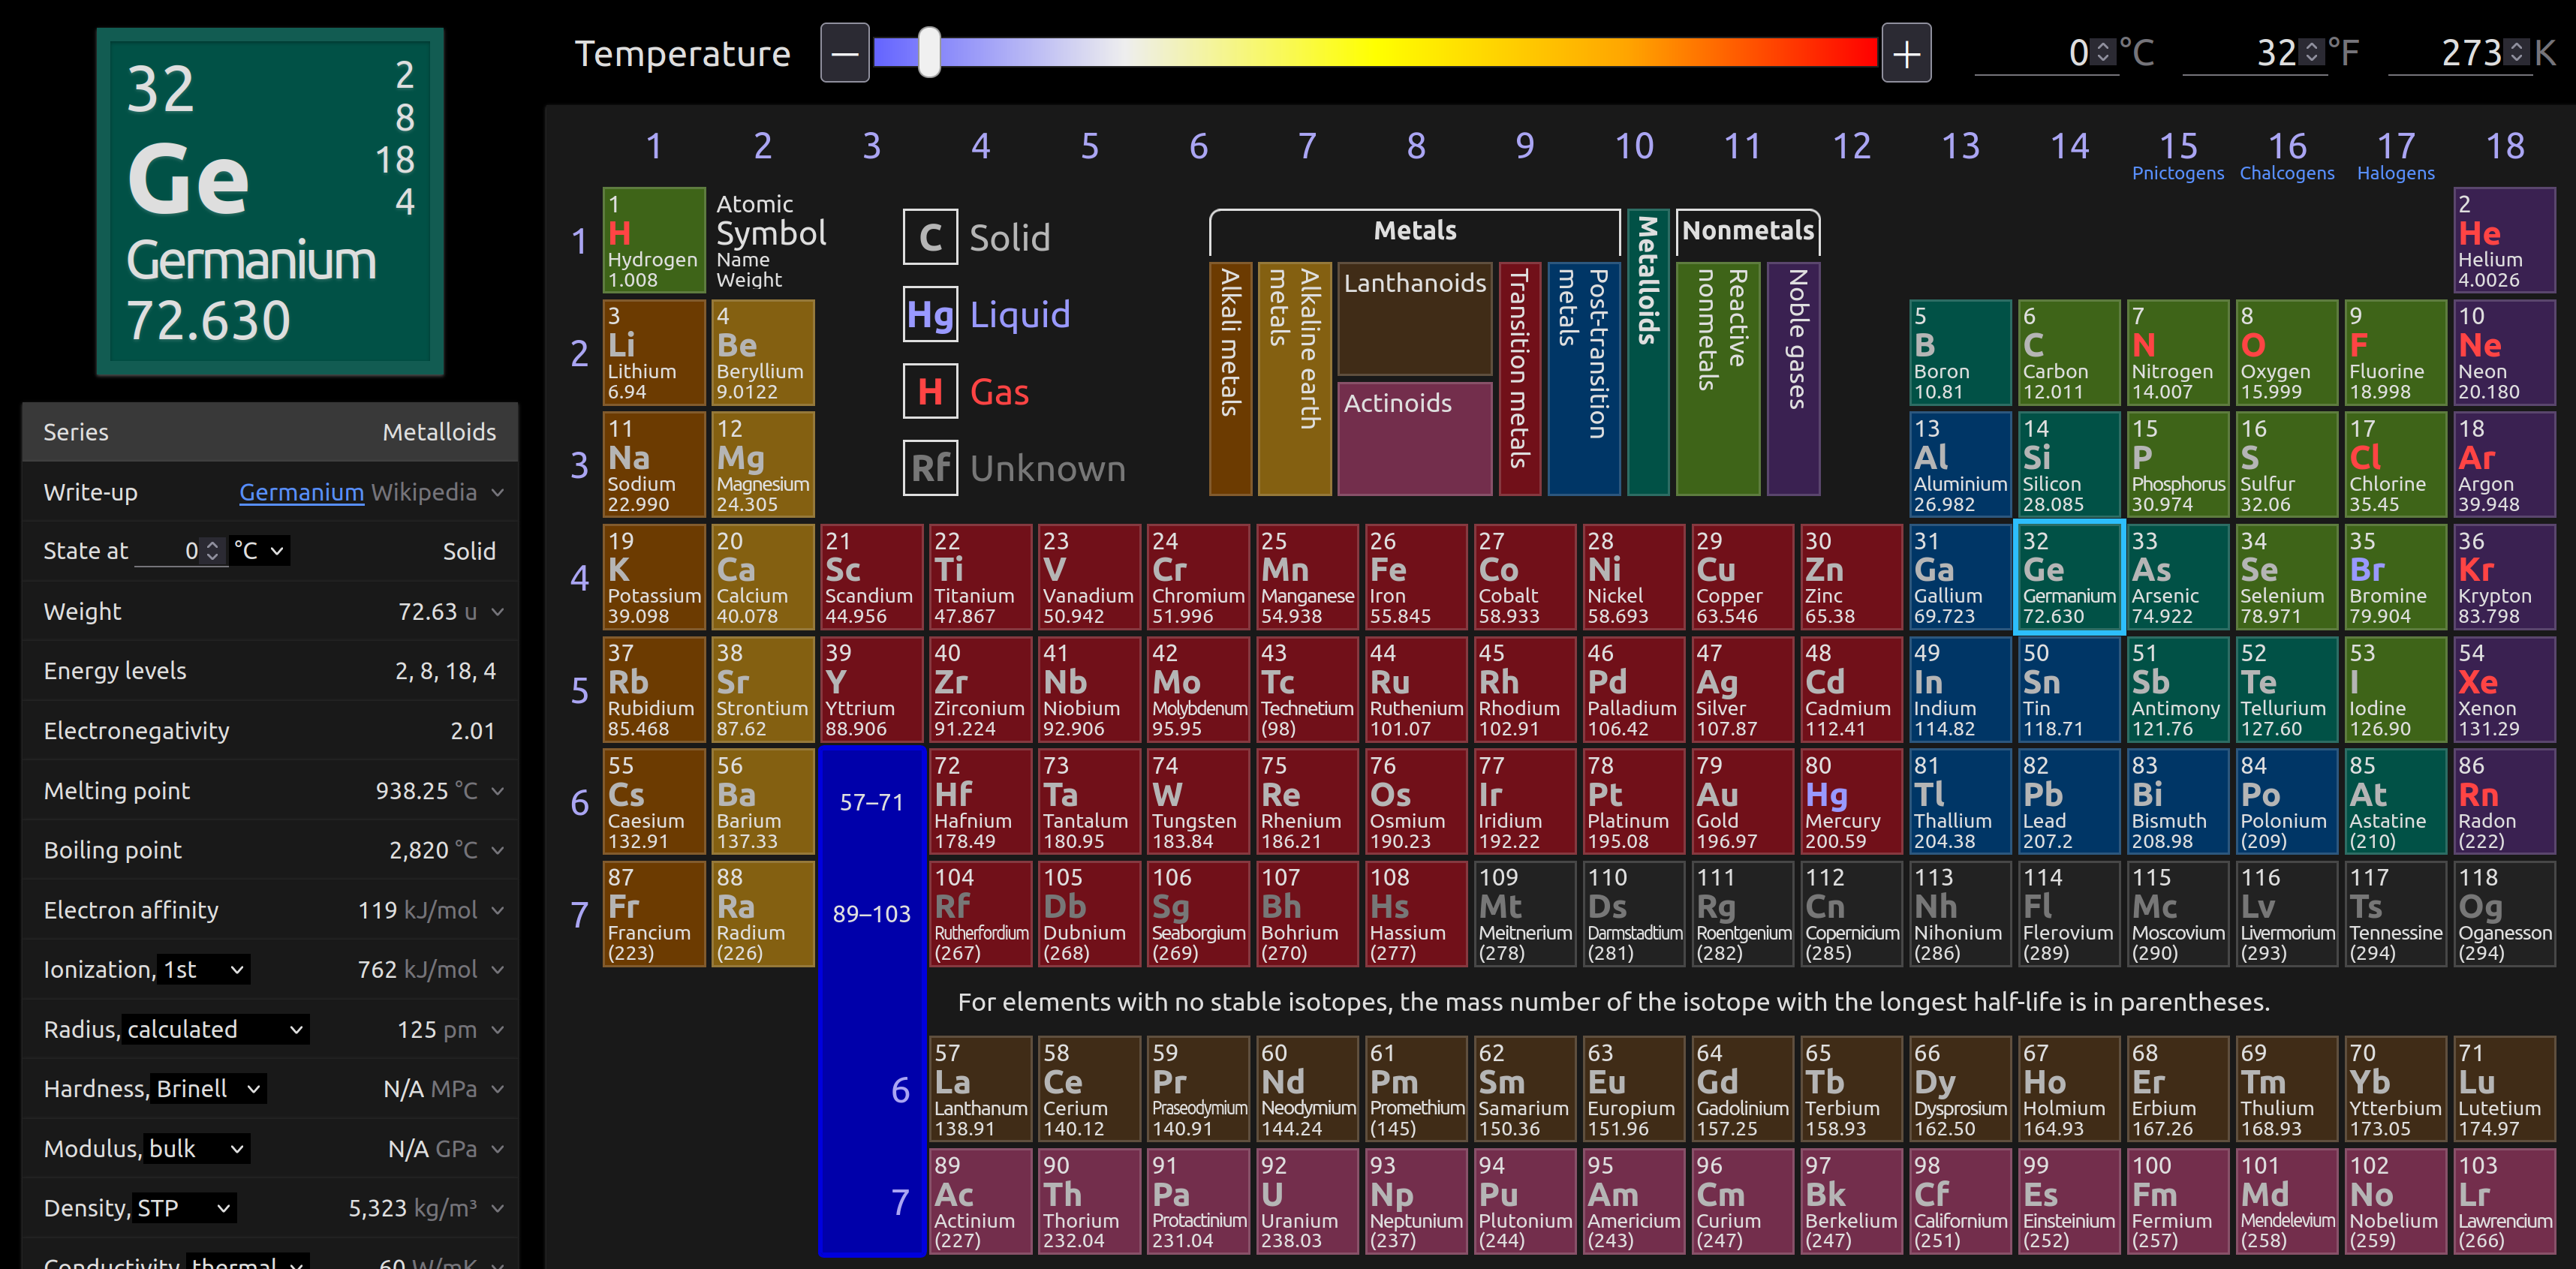
\includegraphics[width=\linewidth]{ptable}

  \textbf{Ge} - 72.630 amu for 1 atom and the molar mass is 72.630 g/mol

  1 amu = $1.66054\times 10^{-24}$ g
\end{frame}

\begin{frame}{Defn: Solvent and Solute}
  \begin{center}
    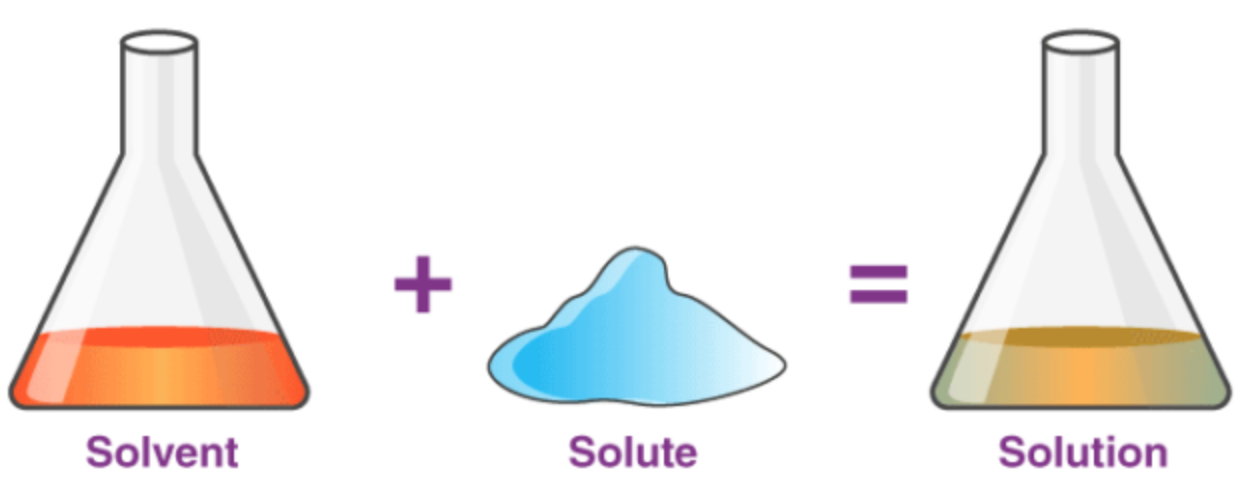
\includegraphics[width=0.75\linewidth]{solut_solv.png}
  \end{center}

  \textbf{Solute} - a substance (solid, liquid, or gas) dissolved in
  a solvent

  \textbf{Solvent} - the material (liquid or gas) that dissolves the
  solute
\end{frame}

\begin{frame}{Molarity - Concentration of Solution}
  \textbf{Definition of Molarity}
  \begin{align}
    M = \frac{n_\text{solute}}{V}
  \end{align}

  where $M$ is molarity, $n_\text{solute}$ is the mols of solute, and $V$ is volume in L

  \textbf{Q:} What is the units for molarity $M$?
\end{frame}

\begin{frame}{Diluting Solutions}
  \begin{center}
    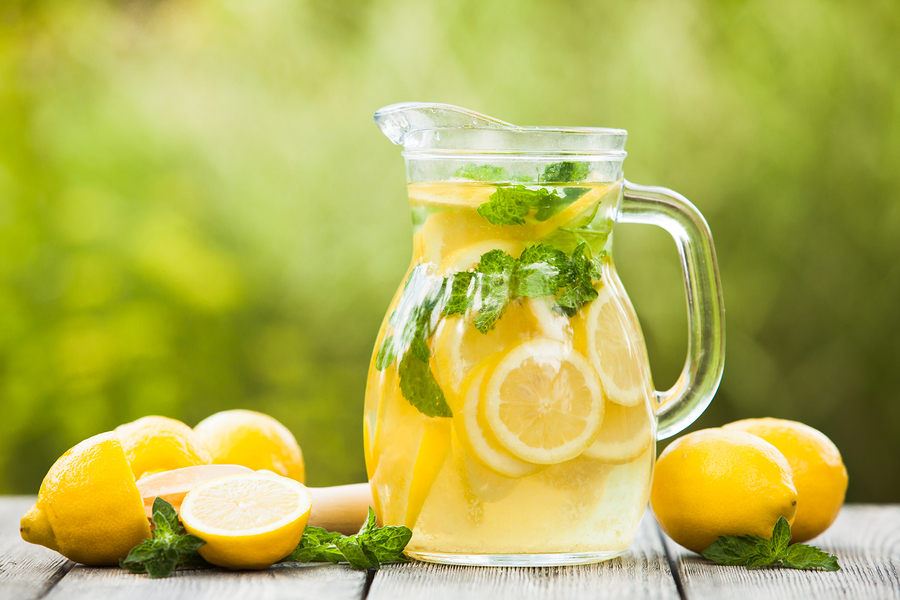
\includegraphics[width=0.4\linewidth]{lemonade}
  \end{center}
  
  Dilution is the process that makes a solution less concentrated. Example is
  lemonade tasting too sweet.

  \textbf{Q:} For given concentrated solution at molarity $M_1$ and a given volume $V_1$, does
  diluting the solution to a new concentration $M_2$ and volume $V_2$ change the amount of mols
  present?
\end{frame}

\section{Chemical Reactions}

\begin{frame}{Chemistry is Everywhere!}
  \centering
  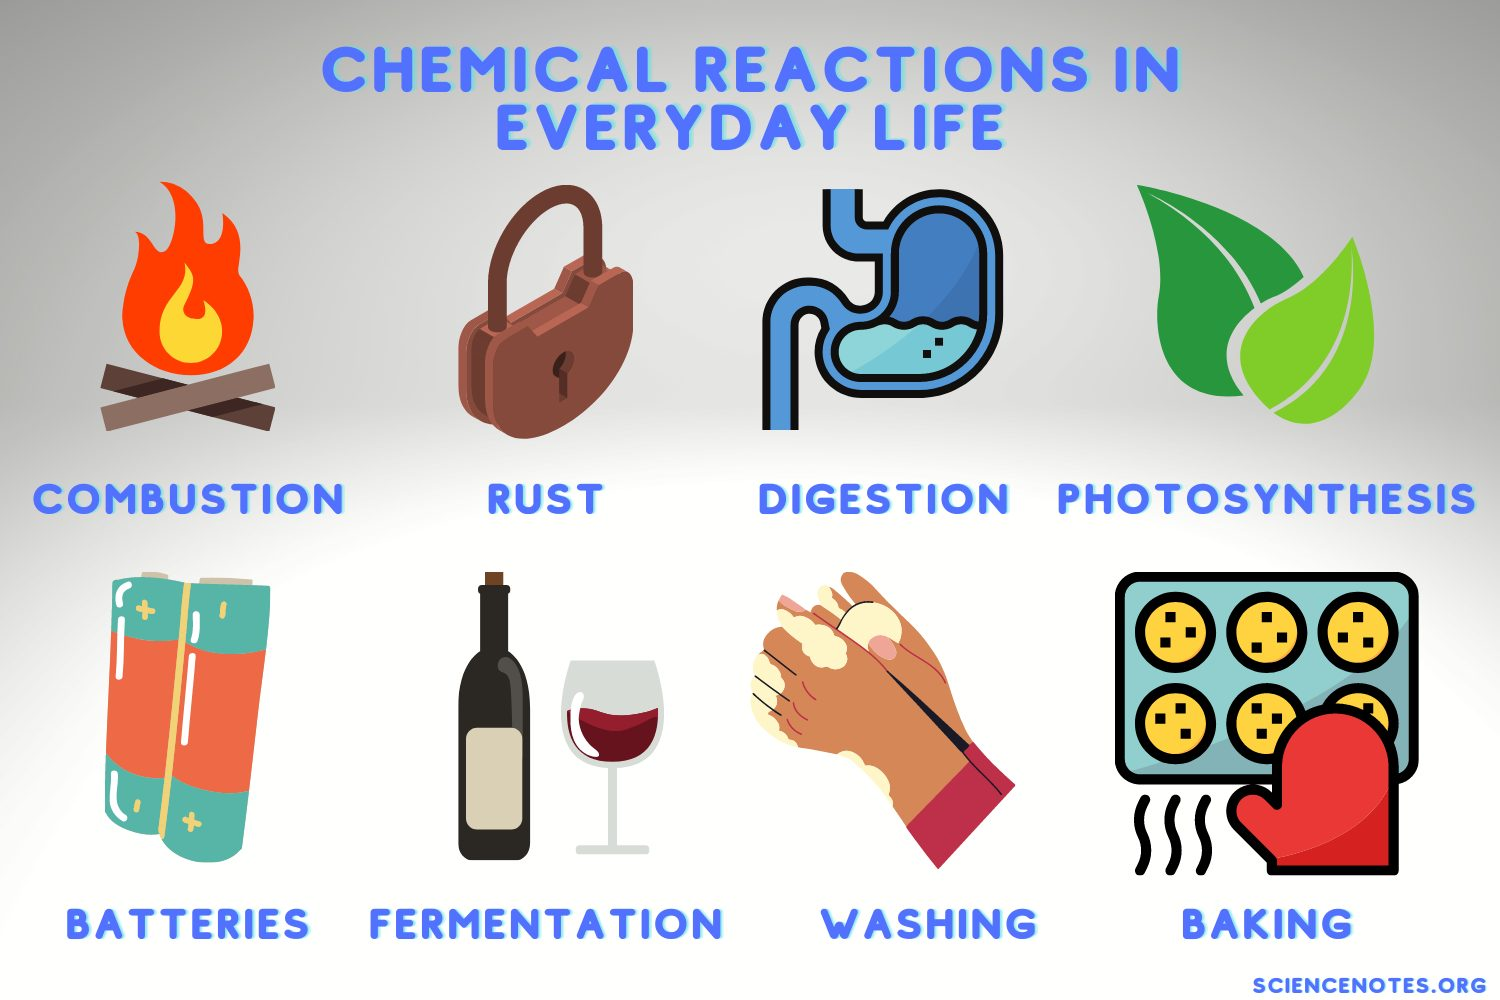
\includegraphics[width=\linewidth]{chem_reactions}
\end{frame}

\subsection{Signs of a Chemical Reaction}

\begin{frame}{Defining a Chemical Reaction}
  \begin{equation}
    A + B \rightarrow C + D
    \label{eqn:chem}
  \end{equation}

  \begin{itemize}
  \item Reactants - chemicals that we start with ($A$ and $B$)
  \item Products - chemicals that are formed after ($C$ and $D$)
    a reaction
  \end{itemize}

  \onslide<2->{\textbf{Q:} Based on Eqn \ref{eqn:chem}, can the reaction go
  in the reverse e.g. $C$ and $D$ turning into $A$ and $B$? Why
  and why not?}
\end{frame}

\begin{frame}{Indications of a Chemical Reaction}
  \begin{center}
    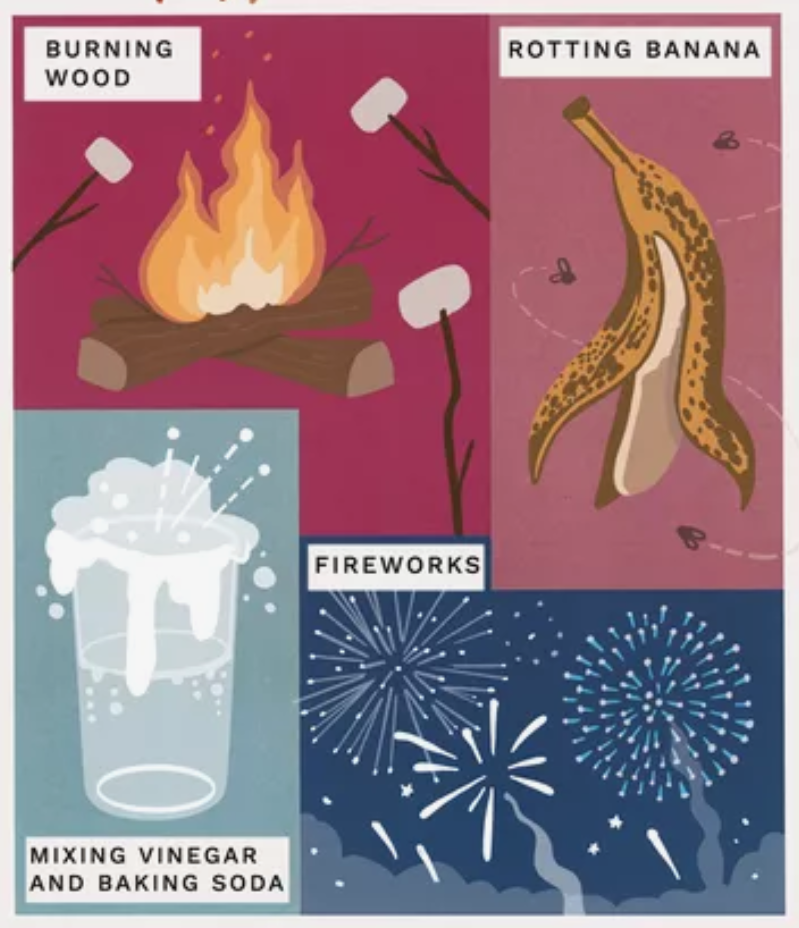
\includegraphics[scale=0.15]{chem_change}
  \end{center}

  \begin{itemize}
  \item Change in color
  \item Production of light
  \item Formation of a solid e.g. precipitate
  \item Formation of a gas
  \item Absorption or release of heat
  \end{itemize}
\end{frame}

\subsection{Writing and Balancing Chem Equations}

\begin{frame}{Writing and Balancing Chem Equations}
  \textbf{Definitions:}

  Chemical equation - symbolic representation of a chemical
  reaction

  Balanced equation - draws upon the conservation of mass; the
  mass of the reactants and the masst of products are equal

  \onslide<2->{\textbf{Q:} Are the moles of reactants and the
    moles of products the same?}
\end{frame}

\begin{frame}{Example: Balancing Chem Equation}
  Balance the following chemical equations:

  \begin{enumerate}[(a)]
  \item CaCl$_2$(aq) + Na$_2$SO$_4$(aq) $\rightarrow$
    CaSO$_4$(s) + NaCl(aq)
  \item[]
  \item CaO(s) + H$_2$O $\rightarrow$ Ca(OH)$_2$(aq)
  \item[]
  \item N$_2$(g) + Mg(s) $\rightarrow$ Mg$_3$N$_2$(s)
  \item[]
  \item CH$_4$(g) + O$_2$(g) $\rightarrow$ CO$_2$(g) + H$_2$O(g)
  \end{enumerate}
  
\end{frame}

\section{Predicting Chemical Reactions}

\subsection{Classes of Reactions}

\begin{frame}{Classes of Reactions}
  \footnotesize
  \begin{table}[hbpt]
    \centering
    \begin{tabular}{c|ccc}
      Class & Reactants & Products & Example \\
      \hline\hline
      Decomposition & 1 compound & multiple   & CD $\rightarrow$ C + D \\
      Combination   & multiple   & 1 compound & A + D $\rightarrow$ AD \\
      Single-displacement & elem+comp & elem+comp & A + CD $\rightarrow$ C +AD\\
      Double-displacement & 2 compounds & 2 compounds & AB + CD $\rightarrow$ AD + BC
    \end{tabular}
  \end{table}
\end{frame}

\begin{frame}{Decomposition Reactions}
  \begin{equation}
    \text{CD} \rightarrow \text{C} + \text{D}
  \end{equation}
  \begin{itemize}
  \item Breaks down compounds into simpler compounds and/or elements
  \item Often the breakdown involves the use of heat e.g. breaking the
    bonds
  \end{itemize}
\end{frame}

\begin{frame}{Examples of Decomposition Reactions}
  \textbf{Oxides and Halides of Metals}
  \begin{equation}
    2\text{HgO(s)} \rightarrow 2\text{Hg(l)} + \text{O}_2\text{(g)}
  \end{equation}
  \begin{equation}
    \text{PtCl$_4$(s)} \rightarrow \text{Pt(s)} + 2\text{Cl$_2$(g)}
  \end{equation}
  \textbf{Peroxides}
  \begin{equation}
    2\text{H$_2$O$_2$(aq)} \rightarrow 2\text{H$_2$O(l)} + \text{O$_2$(g)}
  \end{equation}
  \textbf{Metal Carbonates}
  \begin{equation}
    \text{NiCO$_3$(s)} \rightarrow \text{NiO(s)} + \text{CO$_2$(g)}
  \end{equation}
\end{frame}

\begin{frame}{Cont. Examples of Decomposition Reactions}
  \textbf{Oxoacids}
  \begin{equation}
    \text{H$_2$CO$_3$(aq)} \rightarrow \text{CO$_2$(g)} + \text{H$_2$O(l)}
  \end{equation}
  \begin{equation}
    \text{Ca(OH)$_2$(s)} \rightarrow \text{CaO(s)} + \text{H$_2$O(g)}
  \end{equation}
\end{frame}

\begin{frame}{Metal Hydrates}
  A number of compounds that contain water or components of water e.g.
  metal hydrates
  
  \begin{equation}
    \text{CaSO$_4$}\cdot\text{2H$_2$O}\rightarrow \text{CaSO$_4$(s)} + 2\text{H$_2$O(g)}
  \end{equation}

  Anhydrous compound - substances without any water contents
\end{frame}

\begin{frame}{Example: Decomposition Reaction}
  A scientist needs cobalt(II) oxide to make cobalt glass. The available
  compounds are CoCl$_2\cdot 6$H$_2$O, CoCO$_3$, CoS, and Co(OH)$_2$. Which
  of these compounds can make the cobalt(II) oxide needed?
  \onslide<2->{
    \begin{align*}
      \text{CoCO$_3$(s)} \rightarrow & \text{CoO(s)} + \text{CO$_2$(g)} \\
      \text{Co(OH)$_2$(s)} \rightarrow & \text{CoO(s)} + \text{H$_2$O(g)}
    \end{align*}
  }
\end{frame}

\begin{frame}{Combination Reaction}
  \begin{equation}
    \text{A} + \text{D} \rightarrow \text{AD}
  \end{equation}

  \begin{itemize}
  \item When two substances react to produce a single compound
  \item Elements react to form compounds
  \item Compounds can combine to form another compound
  \item Element react with another compound to form another
    substance
  \end{itemize}
\end{frame}

\begin{frame}{Summary of Combination Reactions}
  \textbf{Metal and Nometal}
  \begin{equation}
    2 \text{Na(s)} + \text{Cl}_2\text{(g)} \rightarrow 2 \text{NaCl(s)}
  \end{equation}
  \textbf{Nonmetal and Nonmetal}
    \begin{equation}
      \text{C(s)} + \text{O}_2\text{(g)} \rightarrow \text{CO}_2\text{g}
    \end{equation}
  \textbf{Element and Compound}
    \begin{equation}
      2 \text{CO(g)} + \text{O}_2\text{(g)} \rightarrow 2\text{CO}_2\text{(g)}
    \end{equation}
  \textbf{Compound and Compound}
    \begin{equation}
      \text{CaO(s)} + \text{CO}_2\text{(g)} \rightarrow \text{CaCO}_3\text{(s)}
    \end{equation}
\end{frame}

\begin{frame}{Practice: Combination Reaction}
  When pure calcium metal is exposed to the oxygen in air, white coating appears
  on the surface. Predict the product and write a complete, balanced equation.
  \onslide<2->{
    \begin{equation*}
      2 \text{Ca(s)} + \text{O$_2$(g)} \rightarrow 2 \text{CaO(s)}
    \end{equation*}
  }
\end{frame}

\begin{frame}{Single-Displacement Reaction}
  A single element displaces another element within a compound

  \textbf{Aluminum displacing Fe$_2$O$_3$}
  \begin{equation}
    \text{Al(s)} + 2\text{Fe$_2$O$_3$(s)} \rightarrow \text{Al$_2$O$_3$(s)} + 2\text{Al(l)}
  \end{equation}
  
  \textbf{Metal displaces a hydrogen in water}
  \begin{equation}
    \text{Ca(s)} + 2\text{H$_2$O(l)} \rightarrow \text{Ca(OH)$_2$(s)} + \text{H$_2$(g)}
  \end{equation}
  Recall the alkali earth metals and alkaline earth metals are highly reactive
  species
\end{frame}

\begin{frame}{Metal Reactivity}
  \centering
  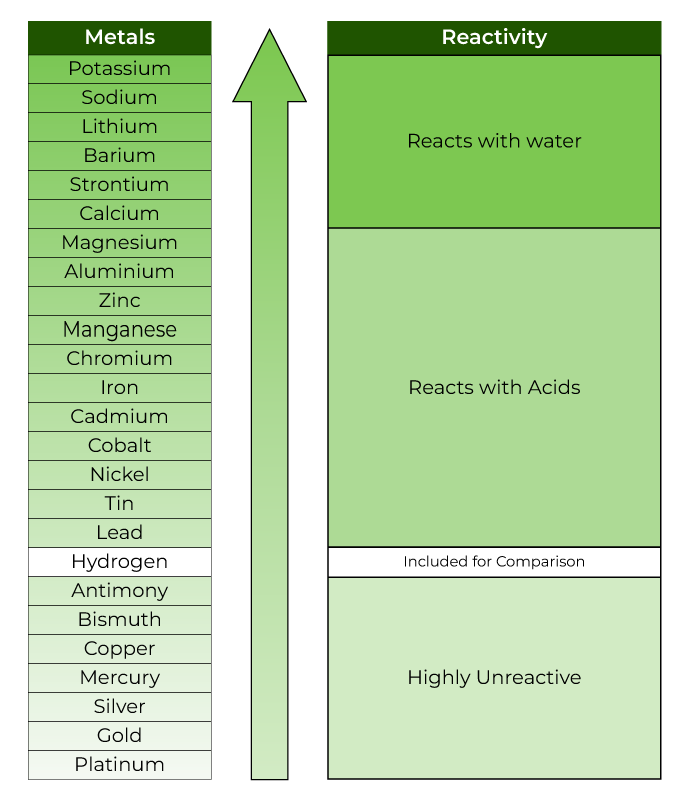
\includegraphics[scale=0.3]{metal_reactivity}
\end{frame}

\begin{frame}{Double-Displacement Reaction}
  A reaction where elements/polyatomic ions within compounds switch places

  \textbf{Precipitation Reaction}
  \begin{equation}
    \text{Pb(CH$_3$CO$_2$)$_2$(aq)} + 2\text{KI(aq)} \rightarrow
    \text{PbI$_2$(s)} + 2\text{KCH$_3$CO$_2$(aq)}
  \end{equation}

  \textbf{Acid-Base Reaction}
  \begin{equation}
    \text{KOH(aq)} + \text{HNO$_3$(aq)} \rightarrow \text{H$_2$O(l)} + \text{KNO$_3$(aq)}
  \end{equation}
\end{frame}

\subsection{Precipitation Rules}

\begin{frame}{Memorize: Precipitation Rules}
  \centering
  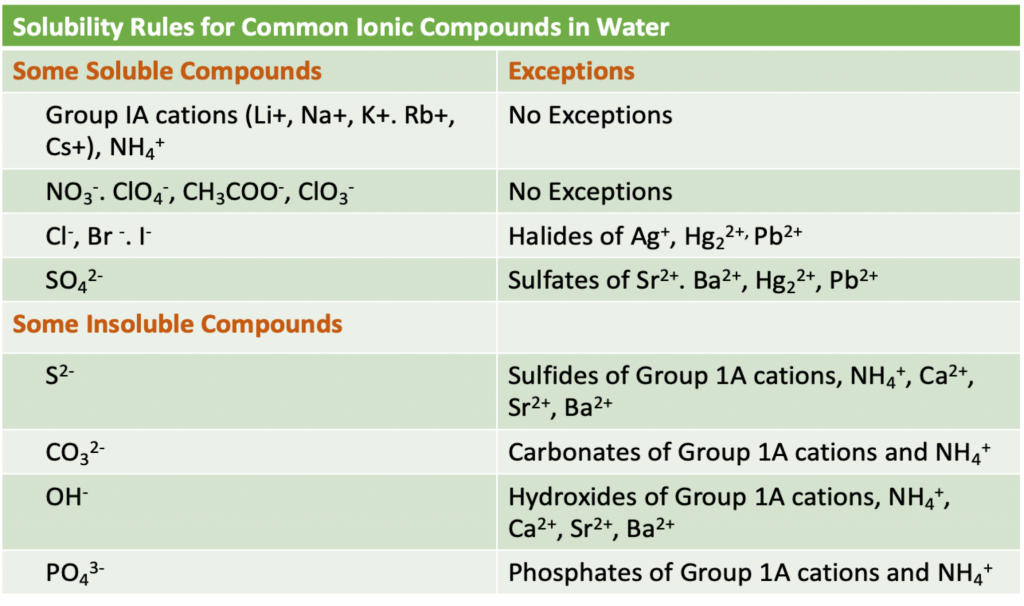
\includegraphics[scale=0.3]{solubility_rules}
\end{frame}

\begin{frame}{Practice: Precipitation Reaction}
  Suppose lead(II) nitrate and potassium chromate solutions are mixed.
  A yellow precipitate begins to appear, identify the precipitate and
  write a balanced equation for the reaction carried out.
  \begin{align*}
    \text{Pb(NO$_3$)$_2$(aq)} + \text{KCrO$_3$(aq)} \rightarrow
    \onslide<2->{\text{PbCrO$_3$(s)} + \text{KNO$_3$(aq)}}
  \end{align*}
\end{frame}

\begin{frame}{Practice: Addt'l Precipitation Reaction}
  Mixing solutions of cadmium(II) nitrate and sodium sulfide lead to an orange
  precipitate. Identify the precipitate and write the balanced equation carried
  out.
  \vfill
\end{frame}

\begin{frame}{Acid-Base Reaction}
  Neutralizes the acidity/basicity of the solution
  \begin{equation}
    \text{HA} + \text{B} \rightarrow \text{A} + \text{HB}
  \end{equation}
  where HA is the acid and B is the base. An example is
  the mixture of Ca(OH)$_2$ and HCl
  \begin{equation}
    \text{Ca(OH)$_2$(aq)} + \text{HCl(aq)} \rightarrow \text{CaCl$_2$(aq)} +\text{H$_2$O(l)}
  \end{equation}
\end{frame}

\begin{frame}{Example: Antacids}
  Upset stomachs are often treated with an acid that is a suspension of
  magnesium hydroxide in water. Stomach acid is hydrochloric acid. Write
  a balanced equation for the reaction between magnesium hydroxide and
  stomach acid
  \onslide<2->{
  \begin{equation}
    2\text{Mg(OH)$_2$(aq)} + 2\text{HCl(aq)} \rightarrow \text{MgCl$_2$(aq)} + 
    2\text{H$_2$O(l)}
  \end{equation}
  }
\end{frame}

\begin{frame}{Combustion Reactions}
  \textbf{Hydrocarbon Combustion} (Majority)
  \begin{center}
    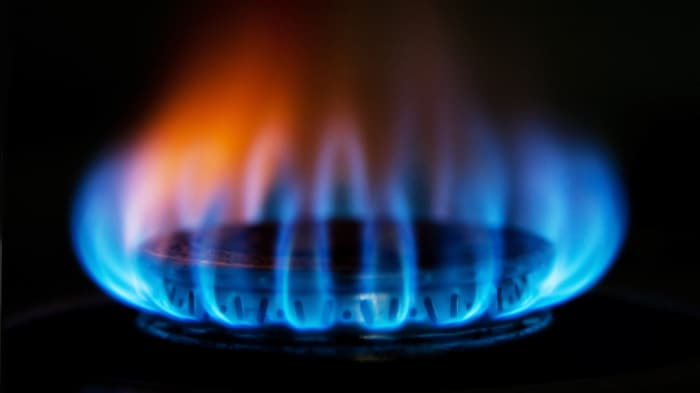
\includegraphics[scale=0.25]{stove_gas}
  \end{center}
  
  Reactions with O$_2$(g) leading to large heat released. Example
  above is the burning of hydrocarbon (C$_x$H$_y$) and follows
  \begin{equation}
    \text{C$_x$H$_y$(g)} + \text{O$_2$(g)} \rightarrow \text{CO$_2$(g)}
    + \text{H$_2$O(g)}
  \end{equation}
\end{frame}

\begin{frame}{Strategy to Balance Hydrocarbon Combustion}
  \begin{enumerate}
  \item Balance carbon and hydrogen on the product side
  \item Balance the oxygen on the reactant side
  \end{enumerate}
\end{frame}

\begin{frame}{Practice: Balancing Hydrocarbon Combustion}
  \begin{enumerate}[(a)]
  \item CH$_4$(g) + O$_2$(g) $\rightarrow$
    CO$_2$(g) + H$_2$O(g)
  \item[]
  \item C$_6$H$_14$(g) + O$_2$(g) $\rightarrow$
    %CO$_2$(g) + H$_2$O(g)
  \item[]
  \item C$_{2}$H$_{5}$OH(l) + O$_2$(g) $\rightarrow$
    %CO$_2$(g) + H$_2$O(g)
  \item[]
  \item NH$_3$(g) + O$_2$(g) $\rightarrow$
    %N$_2$(g) + H$_2$O(g)
  \end{enumerate}
\end{frame}

\begin{frame}{Combustion Reactions}
  \textbf{Metal Combustion}
  \begin{center}
    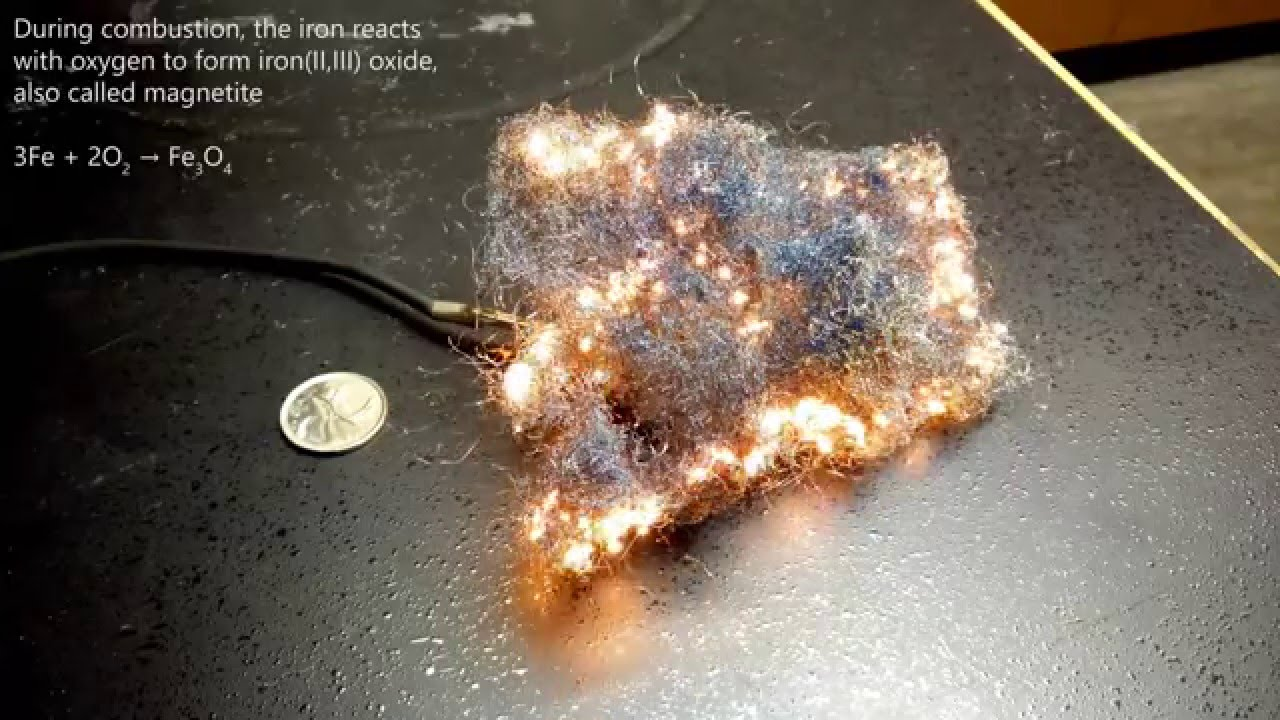
\includegraphics[scale=0.17]{metal_combust}
  \end{center}
  \href{https://www.youtube.com/watch?v=Z2llRM6UYlU}{Iron Combustion Video Link}
\end{frame}

\begin{frame}{Practice: Combustion Reactions}
  Complete and balance the following combustion reactions
  \begin{enumerate}[(a)]
  \item Na(s) + O$_2$(g) $\rightarrow$
    %Na$_2$O(s)
  \item[]
  \item Al(s) + O$_2$(g) $\rightarrow$
    %Al$_2$O$_3$(s)
  \item[]
  \item CO(g) + O$_2$(g) $\rightarrow$
    %CO$_2$(g) + H$_2$O(g)
  \item[]
  \item P$_4$(s) + O$_2$(g) $\rightarrow$
    %N$_2$(g) + H$_2$O(g)
  \end{enumerate}  
\end{frame}

\end{document}
